%----------------------------------------
% Write your notes here
%----------------------------------------

\section{Part 1: Guest Lecture}
In the first part of today's class, we had \c{C}a\v{g}atay Demiralp, reseacher from IBM T. J. Watson Research Center, present on data visualization. You can view his slides \href{https://drive.google.com/file/d/0B-M9UEiE6KFAWmtvUjQta0RFNkk/view}{here}. The following is a summary, although much is borrowed from his slides.

\subsection{What is visualization?}
Why create visualizations? Some examples:
\begin{itemize}
	\item E.J Marey's sphygmograph (Braun 83)
	\item John Snow's mapping of cholera cases on Broad St. (Tufte 83)
	\item Florence Nightingale's Crimean War Deaths (1856)
\end{itemize}
Jacques Bertin, cartographer and theorist, considered \emph{"visualization as the artificial memory"}:
\begin{itemize}
	\item Consider time taken for multiplication by mental calculation vs pen and paper.
	\item Anscombe's quartet: Four datasets have identical summary statistics and linear regression lines, but appear very different when graphed. This is shown in Figure \ref{fig:anscombes_quartet}.
	\begin{figure}[ht]
		\begin{center}
			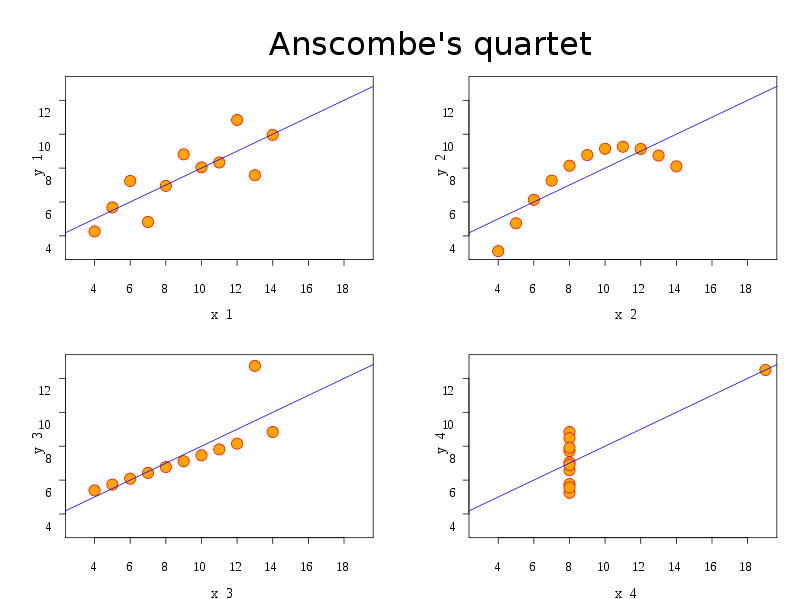
\includegraphics[width=0.5\textwidth]{figures/anscombes_quartet.png}
			\caption{
				Anscombe's quartet - With proper encoding of the data, we are able to make more sense of it.}
			\caption*{Source: Wikipedia.org}
			\label{fig:anscombes_quartet}
		\end{center}
	\end{figure}
	\item Popularity of John W. Tukey (1915-2000) on Wikipedia: After observing the number of page views across time, we notice a spike in January 2011 (Figure \ref{fig:john_tukey}). Why?
	\begin{figure}[ht]
		\begin{center}
			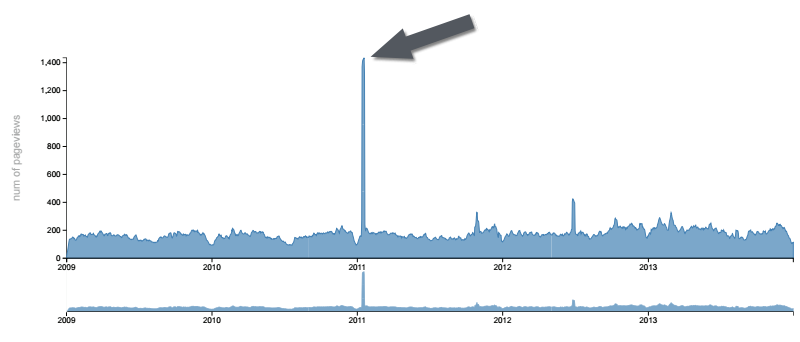
\includegraphics[width=0.5\textwidth]{figures/john_tukey.png}
			\caption{
				Popularity of John W. Tukey on Wikipedia across time.}
			\caption*{Source: \c{C}a\v{g}atay Demiralp}
			\label{fig:john_tukey}
		\end{center}
	\end{figure}
	\begin{itemize}
		\item Jeopardy Final Round $\#$6063 on Wednesday, January 12, 2011: "John Tukey coined this compound word in 1958 saying it was as important as tubes, transistors, wires, tapes..."
		\item Answer: \emph{What is software?}
	\end{itemize}	
\end{itemize}
\textbf{Bottom line:} We create visualizations to
\begin{itemize}
	\item Record information
	\item Analyze data to support reasoning
	\item Communicate information to others
\end{itemize}

\subsection{What is a "good" visualization?}
Visualization specification involves several choices, i.e. graph type, use of color, etc... How much do these choices matter?
\newline \newline
\textbf{Design Principles (Mackinlay 86)}
\begin{itemize}
	\item Expressiveness - A set of facts is \emph{expressible} in a visual language if the sentences (i.e. the visualizations) in the language express all the facts in the set of data, and only the facts in the data. Watch out for visualizations that: 
	\begin{itemize}
		\item Cannot express the facts, e.g. a one-to-many relation cannot be expressed in a single horizontal dot plot
		\item Express facts not in the data, e.g. length of bar in graph says something untrue about the data
	\end{itemize}
	\item Effectiveness - A visualization is more \emph{effective} than another visualization if the information conveyed by one visualization is more readily perceived than the information in the other visualization.
\end{itemize}
\textbf{Design Principles - \emph{animation} (B. Tversky 02)}
\begin{itemize}
	\item Congruence - The structure and content of the external representation should correspond to the desired structure and content of the internal representation.
	\item Apprehension - The structure and content of the external representation should be readily and accurately perceived and comprehended.
\end{itemize}
\textbf{Design Principles \emph{translated}:}
\begin{itemize}
	\item Tell the truth and nothing but the truth.
	\item Use encodings that people decode better.
\end{itemize}

\subsection{Not all visual encoding variables are created equal...}
Stevens Power Law (Figure \ref{fig:stevens_power_law}) describes the relationship between the magnitude of a physical variable and its perceived sensation:
\begin{equation}
S = I^p
\end{equation}
where $S$ is perceived sensation, $I$ is physical intensity, and $p$ is an empirically determined exponent. For example, length (such as comparing the length of bars) is perceived linearly, whereas area (such as comparing the area of circles) is underestimated. Stevens' Power Law predicts bias, not necessarily accuracy.
\begin{figure}[ht]
	\begin{center}
		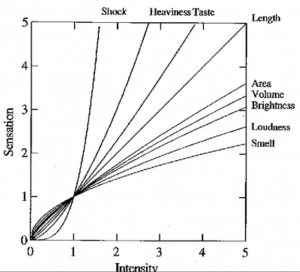
\includegraphics[width=0.5\textwidth]{figures/stevens_power_law.png}
		\caption{
			Stevens' Power Law}
		\caption*{Source: Stevens, S. The psychophysics of sensory function. Am. Sci. 48, 226–253 (1960).}
		\label{fig:stevens_power_law}
	\end{center}
\end{figure} 
\newline
\textbf{Graphical Perception (Cleveland \& McGill 84)}
\begin{itemize}
	\item Task in Experiment I (position - length), Figure \ref{fig:cleveland_mcgill_1}: "For the two marked bars or divisions, what percent the smaller is of the larger?"
	\begin{figure}[ht]
		\begin{center}
			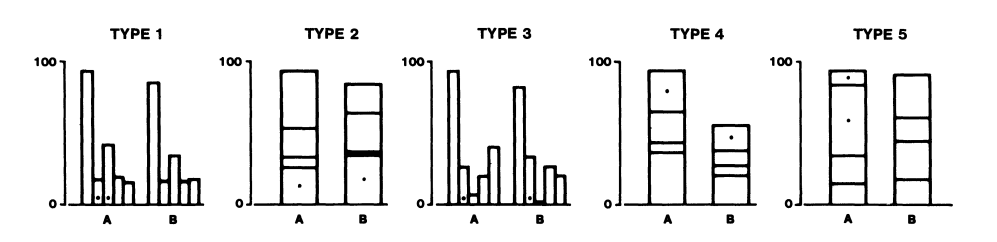
\includegraphics[width=\textwidth]{figures/cleveland_mcgill_1.png}
			\caption{
				Experiment I (position - length)}
			\caption*{Source:  Cleveland, W. \& McGill, R. Graphical perception: Theory, experimentation, and application to the development of graphical methods. J. Am. Stat. 79, 531–554 (1984).}
			\label{fig:cleveland_mcgill_1}
		\end{center}
	\end{figure} \newline
	Type 1, 2, and 3 compare "position" along a common scale, while Type 4 and 5 compare "length". 
	\item Task in Experiment II (position - angle), Figure \ref{fig:cleveland_mcgill_2}: "What percent each of the other segments or bars is of the largest?"
	\begin{figure}[ht]
		\begin{center}
			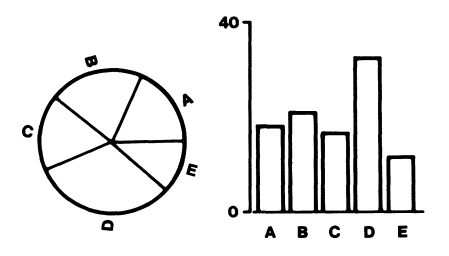
\includegraphics[width=0.4\textwidth]{figures/cleveland_mcgill_2.png}
			\caption{
				Experiment II (position - angle)}
			\caption*{Source: Cleveland, W. \& McGill, R.}
			\label{fig:cleveland_mcgill_2}
		\end{center}
	\end{figure} \newline
	The pie chart on the left compares "angle" while the bar chart on the right compares "position".
	\item Figure \ref{fig:cleveland_mcgill_results} shows the results of Cleveland and McGill's Experiment I (top) and II (bottom). Bias was measured by the log absolute estimation error.
	\begin{figure}[ht]
		\begin{center}
			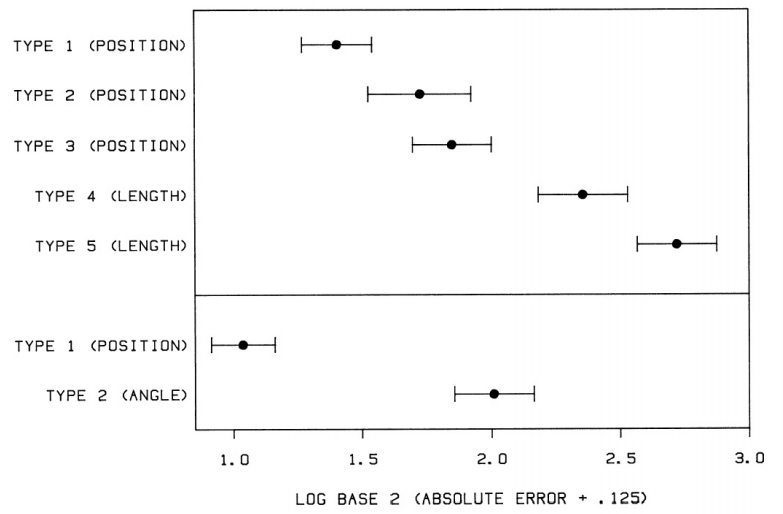
\includegraphics[width=0.8\textwidth]{figures/cleveland_mcgill_results.png}
			\caption{
				Results}
			\caption*{Source: Cleveland, W. \& McGill, R.}
			\label{fig:cleveland_mcgill_results}
		\end{center}
	\end{figure}
\end{itemize}

\subsection{Not all data types are created equal...}
\textbf{Data variable types:}
\begin{itemize}
	\item \emph{Nominal} - has two or more categories, but no instrinsic ordering
	\item \emph{Ordinal} - has two or more categories with natural ordering
	\item \emph{Quantitative} - numerical variables
	\item Mackinlay (86) published effectiveness rankings on the different data variable types.
\end{itemize}

\subsection{Color}
How should I color my bar chart? 
\newline \newline
\textbf{Color Design Guidelines}
\begin{itemize}
	\item Maintain perceptual distinguishability
	\item Use only a few (<7) \& named, when possible
	\item Avoid unintended "pop out" of colors
	\item Get it right in black \& white
	\item Respect cultural norms \& the color blind
	\item Beware of segmentation (rainbows!)
	\item Consider spatial frequency effects
\end{itemize}

\subsection{Tools}
Which tool should I use to create my bar chart?
\begin{itemize}
	\item Tools come and go, but underlying ideas are important
	\item Consider the expressiveness vs the speed of tools
\end{itemize}
\textbf{Declarative languages:}
\begin{itemize}
	\item Programming by describing \emph{what}, not \emph{how}
	\begin{itemize}
		\item In contrast to imperative programming, where you must give explicit steps
	\end{itemize}
	\item Separate specification (what you want) from execution (how it should be computed)
	\item Examples include HTML/CSS, SQL, and D3
	\item Advantages:
	\begin{itemize}
		\item Faster iteration
		\item Less code
		\item Larger user base than imperative languages
		\item Potential to create better visualization - Smart defaults
		\item Reusable - Write-once, then re-apply
		\item Easier programmatic generation - Write programs which output visualizations e.g., automated search \& recommendation
	\end{itemize}	
\end{itemize}
\textbf{The Grammar of Graphics (Wilkinson)}
\begin{itemize}
	\item Algebra is useful! (Sets, operators, rules)
	\begin{itemize}
		\item Operators: + (blend), * (cross), / (nest)
	\end{itemize}
	\item Geometric primitives (marks)
	\begin{itemize}
		\item "Don't give a pie, give primitives to make a pie and more!"
	\end{itemize}
\end{itemize}

\subsection{The Upshot} 
Always consider what the one point you are trying to make with this visualization is. Then, how can you make that point the most obvious thing when your visualization is seen?

\section{Part 2: Intro to ggplot2}
In the second part of today's class, Professor Hofman went over some basic ideas in ggplot2 and how to effectively use visualization tools like ggplot2 to convey a point. To do this, we revisited the Movielens data from Lecture 2. You can find his code in \href{https://github.com/jhofman/msd2017/blob/master/lectures/lecture_5/visualization_with_ggplot2.ipynb}{this Jupyter notebook}. The following are some pointers and best practices that Professor Hofman mentioned throughout the demo:
\begin{itemize}
	\item Convert timestamps to datetime objects using package \emph{lubridate} for easy manipulation
	\begin{itemize}
		\item For example, \verb|year(datetime_object)| can quickly extract the year
	\end{itemize}
	\item General idea of ggplot2: \\
	\verb|ggplot(<dataframe>, 'aes' aesthetic-mapping('x' variable = column_name)) + geom_type|
	\item Use piping operator \verb|%>%| (similar to command line) so that code is easier to follow
	\begin{itemize}
		\item But in ggplot2, remember to use \verb|+| to precede \verb|geom_histogram/geom_point/geom_line| etc. instead of \verb|%>%| because geoms implicitly compute y variable counts.
	\end{itemize}
	\item If x is categorical, i.e. \verb|as.factor(rating)|, ggplot will automatically bin by category instead of breaking up by numerical  intervals
	\item \verb|scale_y_continuous(label = comma)| adds commas to give you easily readable numbers on your y axis
	\item Good practice for making a plot with discrete data: Plot data as points, your model as the line, and optional confidence band as an underlying shade
	\item Changing the window of your data:
	\begin{itemize}
		\item Using \verb|coord_cartesian(xlim = c(starting_value, ending_value))| will only change the visual window of your graph, not the data your graph is using
		\item Use \verb|xlim(c(starting_value, ending_value)| instead, which limits your data before any transformation occurs
	\end{itemize}
	\item Be careful when ignoring warnings!
	\item Playing around with log scales may give the data a completely different story
	\item \verb|geom_density(fill = <color>)| can be used to smooth and fill the area under a graph
	\item Consider using a vertical bar to depict mean: \verb|geom_vline(aes(intercept = mean(num_ratings)),| \\
	\verb|linetype = 'dashed')|
	\item Keep in mind when you are specifying something constant (which you would want to keep outside the aesthetic mapping) vs transforming something IN the data (keep inside the aesthetic mapping)
	\item \verb|cumsum| gives a running sum of values down the column, whereas \verb|sum| gives one value
	\item \verb|coord_flip| is good for seeing long x-axis labels like movie titles
	\item Be aware of the ordering of factors (\verb|mutate(title = reorder(title, mean_rating)))|)
	\item Every design choice depends on the point you want to make!!
	\item If you want to split up data and visualize individual plots together, you can use \verb|title| to break out facets: \verb|facet_wrap(~ title)|
	\item Add standard errors to a line graph with \verb|geom_ribbon|
	\item \verb|extract| can pull out specific texts (regex)
\end{itemize}



%Figure \ref{fig:example_figure} is an example of how to include an image.
%
%\begin{figure}[ht]
%  \begin{center}
%    
\includegraphics[width=0.5\textwidth]{figures/example_figure.png}
%    \caption{
%      This is how to include a figure.
%      As long as you use pdflatex most file types (e.g., jpg, png, pdf) should work.}
%    \label{fig:example_figure}
%  \end{center}
%\end{figure}
%
%And here's some math:
%\begin{equation}
%  \int_{-\infty}^{+\infty} e^{-x^2} dx = \sqrt{\pi}
%\end{equation}
%
%You can also make numbered lists:
%\begin{enumerate}
%  \item Thing 1
%  \item Thing 2
%  \item etc.
%\end{enumerate}
%
%Or bulleted lists
%\begin{itemize}
%  \item Thing 1
%  \item Thing 2
%  \item etc.
%\end{itemize}
%
%It shouldn't get much more complicated than that.
